\chapter{Détermination du diamètre optimal des intervalles à considérer pour l'estimation de la régularité locale }
\minitoc%


Nous avons désormais établi que la génération d'un $\operatorname{FAR}(1)$ basé sur un mouvement brownien multi-fractionnaire permettait de contrôler de bout-en-bout la régularité du processus. Ceci va nous permettre de pouvoir analyser correctement le comportement du risque d'estimation de la régularité en fonction de $\Delta$, ainsi que le comportement du $\Delta^*$ optimal.

\section{Choix des paramètres de la simulation des $\operatorname{FAR}(1)$ localement Hölderiennes}

\info{
	Il est conseillé de se référer aux tableaux [Notations-Spécifique au stage]
	%\ref{tab:notation-specifique-stage} 
	et \ref{tab:model} pour la signification des notations déjà introduites et utilisées dans ce chapitre.
}

\subsection{Nombre de simulations}

Afin d'étudier la relation entre le $\Delta$ optimum et différentes quantités caractéristiques aux données, on va effectuer une simulation de monte carlo.

On décide de générer $\mathsf{mc} = 200$ simulations de Monte-Carlo, afin d'obtenir les résultats les plus robustes possibles pour l'estimation du risque $\esperance{\distnorme 2 {\widehat \Theta} {\widetilde \Theta}}$, tout en gardant un temps de calcul raisonnable. On fait varier $\lambda$ de $30$ à $480$ en incrémentant de $15$ à chaque fois. L'idée et de pouvoir regarder si il existe une relation entre $\Delta^*$ et la position du nombre moyen de points observés apr courbe $(\lambda)$ par rapport au nombre de courbes $(N)$.

\smallskip

Il est possible de voir comment les paramètres que l'on va définir sont utilisés dans l'implémentation en annexe \ref{annexe:code}.


\newcommand{\tlnm}{T^{[\lambda]}_{n}[m]}
\newcommand{\mset}{\llbracket 1, M_n \rrbracket}
\newcommand{\nset}{\llbracket 1, N \rrbracket}
\newcommand{\lbdset}{\llbracket 30, 45, \dots , 480 \rrbracket}
\newcommand{\genxset}{\bigl(\tlnm, X_n(\tlnm)\bigr)_{m \in \mset}}
\newcommand{\simset}{\left\{ \genxset \, : \, n \in \nset, \, \lambda \& N \textsf{ fixés } \right\}}
\newcommand{\simsetall}{\left\{ \genxset \, : \, N \in \overrightarrow N, \, \lambda \in \lbdset, \, n \in \nset \right\}}

\subsection{Fonction de Hurst}

\begin{minipage}{0.47\linewidth}
	On appelle $H : t \mapsto H_t$ la fonction de Hurst. Celle qui a été choisie est la suivante :

	$$
		H^{[0.4, 0.8, 5, 0.5]}_{\textsf{logistic}} : \begin{array}{ccc}
			[0,1] & \longrightarrow & [0.4, 0.8]
			\\
			t     & \longmapsto     & 0.4 + \frac{(0.8 - 0.4)}{1 + e^{-5(t - 0.5)}}
		\end{array}
	$$

	On dispose donc d'une régularité locale qui varie sur $\mathcal T$, tout en ayant une évolution pas trop brusque. Nous allons étudier le comportement du $\Delta$ lors de l'estimation de la régularité locale en les points suivants :

	$$
		\vec t = \begin{bmatrix} 0.3 \\ 0.4 \\ 0.5 \\ 0.6 \\ 0.7 \\ 0.8 \end{bmatrix}
		\quad\quad
		H(\, \vec t \,) =
		\begin{bmatrix}
			0.51 \\ 0.55 \\ 0.6 \\ 0.65 \\ 0.69 \\ 0.73
		\end{bmatrix}
	$$

\end{minipage}
\hfill
\begin{minipage}{0.47\linewidth}
	\begin{figure}[H]
		\centering
		\begin{tikzpicture}
			\begin{axis}[
					width=\textwidth,
					xlabel=$t$,
					ylabel={$H^{[0.4, 0.8, 5, 0.5]}_{\textsf{logistic}}(t)$},
					xmin=0, xmax=1,
					ymin=0.4, ymax=0.8,
					axis lines=center,
					axis on top=true,
					domain=0:1,
					samples=100,
					legend style={at={(0.5,-0.15)},anchor=north},
					legend entries={Fonction de Hurst, Points d'estimation de la régularité locale},
				]
				\addplot [mark=none,smooth,blue] {0.4 + (0.8 - 0.4)/(1 + exp(-5*(x - 0.5)))};
				\addplot [only marks,mark=*] coordinates {
						(0.3,0.51)
						(0.4,0.55)
						(0.5,0.6)
						(0.6,0.65)
						(0.7,0.69)
						(0.8,0.73)
					};
			\end{axis}
		\end{tikzpicture}
		\caption{Hurst Function : Logistic}
		\label{plot:hurst-logistic}
	\end{figure}
\end{minipage}


\subsection{Constante de Hölder
}

On décide de simuler des mouvements browniens multi-fractionnaires de constante de Hölder $L_t$ identique sur tout le support.

$$\forall t \quad L_t = 1$$


\subsection{Moyenne}


\begin{minipage}{0.47\linewidth}

	La fonction moyenne du processus utilisée pour la simulation est la suivante :

	$$
		\mu : \begin{array}{ccc}
			[0,1] & \longrightarrow & \mathbb R
			\\
			t     & \longmapsto     & 4 \cdot \sin\bigl( \frac 3 2 \pi \cdot t \bigr)
		\end{array}
	$$
\end{minipage}
\hfill
\begin{minipage}{0.47\linewidth}
	\begin{figure}[H]
		\centering
		\begin{tikzpicture}
			\begin{axis}[
					width = \textwidth,
					xlabel=$t$,
					ylabel=$\mu(t)$,
					xmin=0, xmax=1,
					ymin=-4, ymax=4,
					axis lines=center,
					axis on top=true,
					domain=0:1,
					samples=100
				]
				\addplot [mark=none,smooth,blue] {4*sin(deg(3/2*pi*x))};
			\end{axis}
		\end{tikzpicture}
		%\caption{Mean function : $\mu(t) = 4 \cdot \sin\bigl( \frac 3 2 \pi \cdot t \bigr)$}
		\label{plot:mu}
	\end{figure}
\end{minipage}







\subsection{Noyau de la relation FAR(1)}
\begin{minipage}{0.48\linewidth}
	On décide de simuler un FAR(1) basé sur un opérateur linéaire intégral :

	$$
		X_{n+1} = \phi(X_n) + \varepsilon_{n+1}
	$$

	avec : $\phi : f \mapsto \displaystyle\int_{\mathcal T} f(u) \beta(u, \cdot \,) \, du$

	C'est une modélisation fréquente des FAR(1). Le noyaux que l'on considère dans l'opérateur intégral pour les simulations est le suivant :


	$$
		\beta : \, \begin{array}{ccc}
			[0,1]^2 & \longrightarrow & \mathbb R
			\\
			(t,s)   & \longmapsto     & \frac 9 4 t\sqrt{ s(1-s) }
		\end{array}
	$$

\end{minipage}
\hfill
\begin{minipage}{0.48\linewidth}
	\begin{figure}[H]
		\centering
		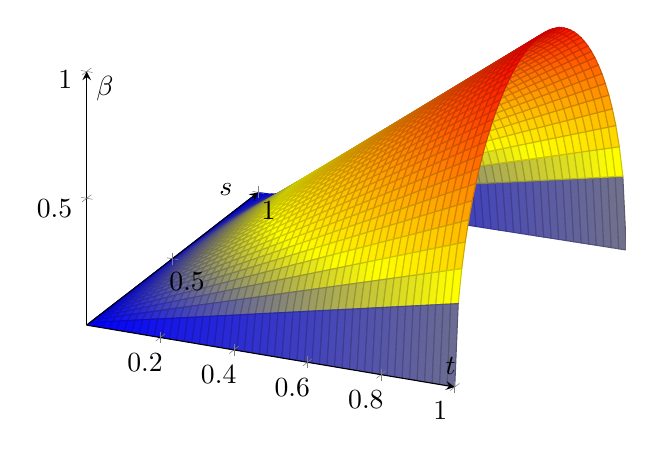
\begin{tikzpicture}
			\begin{axis}[
					xlabel=$t$,
					ylabel=$s$,
					zlabel=$\beta$,
					xmin=0, xmax=1,
					ymin=0, ymax=1,
					zmin=0, zmax=1,
					axis lines=center,
					axis on top=true,
					domain=0:1,
					samples=50,
				]
				\addplot3 [surf] {9/4*x*sqrt(y*(1-y))};
			\end{axis}
		\end{tikzpicture}
		\caption{Graphique du noyau intégral pour la relation FAR(1)}
		\label{graph:far_kernel}
	\end{figure}
\end{minipage}

\bigskip

On notera que le noyaux utilisé pour la relation de $\operatorname{FAR}(1)$ est une fonction lisse. Ainsi il remplit aisément la condition pour que le $\operatorname{FAR}(1)$ hérite de la régularité du mouvement brownien multi-fractionnaire généré.

\subsection{Nombre de courbes}

Afin d'étudier le lien potentiel qu'il pourrait y avoir entre le nombre de courbes observées et le $\Delta$ optimal pour l'estimation de la régularité locale, on choisit plusieurs valeurs de nombres de courbes observées de telle sorte à avoir un \og petit \fg et un \og grand \fg nombre de courbes observées.

On choisit les valeurs suivantes concernant le nombre de courbes observées :

$$
	\vec N = [ 100, 200, 300, 400]
$$

Ainsi on traîte les cas de ce qu'on pourrait considérer comme la limite avant d'entrer dans un cas \og sparse \fg (en terme du nombre d'observations de courbe), jusqu'à un nombre de courbe que l'on peut considérer important.

\subsection{Nombre moyen de points observés par courbe}

Le nombre de points observés sur la courbe $X_n$ est défini comme étant la variable aléatoire $M_n$. Dans le cadre de notre simulation, $M_n$ suit une loi de poisson de paramètre $\lambda$. Ainsi, $\esperance{M_n} = \lambda$ dans le cadre de notre simulation.

On effectue ainsi une simulation d'un échantillon de série temporelle $\operatorname{FAR}(1)$ par nombre moyen de points que l'on souhaite observer sur les courbes ($\lambda$). Afin de traîter différents cas, d'observation \og dense \fg à observation \og sparse \fg (dans le sens du nombre de points par courbe), on fait varier $\lambda$ de $30$ points par courbe en moyenne à $480$ points. L'idée est de voir ensuite si il y a une relation entre le $\Delta^*$ et le fait que l'on ait $\lambda$ petit, similaire ou grand par rapport à $N$.

\subsection{Ensemble des $\Delta$ testés}

On souhaite obtenir plusieurs graphiques avec $\Delta$ sur l'axe des abscisses afin de pouvoir étudier le comportement de diverses quantitées, dont le risque euclidien, lorsque l'on fait varier $\Delta$ avec certains paramètres fixés (nombre de courbes observées, nombre moyen de points observés par courbe, ...). Toutefois plus on va considérer de $\Delta$, et plus la simulation sera coûteuse. En effet, on a vu en section \ref{rem:inversion_matrice_covariance_mfbm_informel} que l'odre de complexité de la simulation du mfBm est de $\mathcal O \bigl( \operatorname{card} T^3 \bigr)$, avec $T$ les points où l'on doit évaluer nos $\famfinie X 1 n$. Dans notre cas, le nombre de points considérés pour la simulation est :

$$\underbracket[0.187ex]{\dim \vec\Delta}_{30} \times \underbracket[0.187ex]{3}_{t_1 / t_2 / t_3} \times \underbracket[0.187ex]{\dim \vec t}_{6} + \underbracket[0.187ex]{n_{Grid\_\int}}_{100} + \underbracket[0.187ex]{\lambda}_{\leq 480} \leq \underbracket[0.187ex]{640}_{fixe} + \underbracket[0.187ex]{480}_{pts \, aleat} = 1 \, 120$$

% Afin d'avoir une approximation correcte de l'intégrale requise pour la relation FAR(1), on choisit d'effectuer la méthode des rectangles en découpant $[0,1]$ en 100 sous intervalles réguliers. On a besoin aussi d'évaluer la vraie valeur des $X_i$ en $t_1, t_2, t_3$ et ce, pour chaque valeur de $\Delta$ afin de pouvoir comparer l'estimateur $\hat \theta(u,v) = \frac 1 N \sum_i (\widehat X_i(u) - \widehat X_i(v))^2$ obtenu via le pré-lissage avec la valeur intangible $\tilde \theta(u,v) = \frac 1 N \sum_i ( X_i(u) -  X_i(v))^2$; et ce sur l'ensemble des différents points $t_2 \in \vec t$


Pour assurer un équilibre entre le nombre de points et les temps de simulation, nous choisissons 30 valeurs uniformément réparties entre 0.01 et 0.2 pour $\Delta$. Au-delà de cette plage, la largeur des intervalles pour l'évaluation de la régularité devient disproportionnée par rapport à la taille du support, rendant inappropriée la notion de \og régularité locale \fg.
$$
	\vec \Delta = \left[ 0.01 \cdots  0.2 \right]_{30}
$$

\subsection{Bruit blanc}


Une fois que l'on a simulé :

$$
	\famfinie X 1 n \quad \textsf{vérifiant} \quad X_{n+1} = \phi(X_n) + \xi_n
$$

on doit désormais reproduire l'erreur de mesure, pour cela chaque courbe est ensuite bruitée en rajoutant un bruit blanc :

$$
	\eta \sim \mathcal N ( 0, 0.04 )
$$

Il est important d'avoir un bruit blanc d'écart type d'un ordre de grandeur en dessous de celui des valeurs prises par le processus, sinon l'estimation serait mauvaise quoi qu'il arrive. En effet le bruit écraserait à lui tout seul toute l'information fine de régularité.


\subsection{Résumé des Paramètres}

\begin{table}[H]
	\centering
	\begin{tabular}{l|l|ll|l|}
		\cline{2-5}
		\textbf{}                                                                  & \textbf{nombre de valeurs testées} & \multicolumn{1}{l|}{\textbf{de}} & \textbf{jusqu'à}         & \textbf{valeur}          \\ \hline
		\multicolumn{1}{|l|}{\textit{\textbf{$\Delta$}}}                           & $30$                               & $0.01$                           & $0.2$                    & \cellcolor[HTML]{C0C0C0} \\
		\multicolumn{1}{|l|}{\textit{\textbf{$\lambda$}}}                          & $30$                               & $30$                             & $480$                    & \cellcolor[HTML]{C0C0C0} \\
		\multicolumn{1}{|l|}{\textit{\textbf{$N$}}}                                & $4$                                & $100$                            & $400$                    & \cellcolor[HTML]{C0C0C0} \\
		\multicolumn{1}{|l|}{\textit{\textbf{Erreur de mesure : ($\sigma_\eta$)}}} & \cellcolor[HTML]{C0C0C0}           & \cellcolor[HTML]{C0C0C0}         & \cellcolor[HTML]{C0C0C0} & $0.2$                    \\
		\multicolumn{1}{|l|}{\textit{\textbf{nb simulations MC}}}                  & \cellcolor[HTML]{C0C0C0}           & \cellcolor[HTML]{C0C0C0}         & \cellcolor[HTML]{C0C0C0} & $200$                    \\ \hline
	\end{tabular}
	\caption{Hyper-paramètres de la simulation Monte-Carlo}
	\label{tab:hyperparam-mc}
\end{table}


\section{Prélissage des données simulées}

\subsection{Les courbes obtenues}

Voici l'exemple d'une courbe obtenue (courbe 1, 99$^{eme}$ simulation de monte-carlo) :

\begin{figure}[H]
	\centering
	\textbf{Données simulées}

	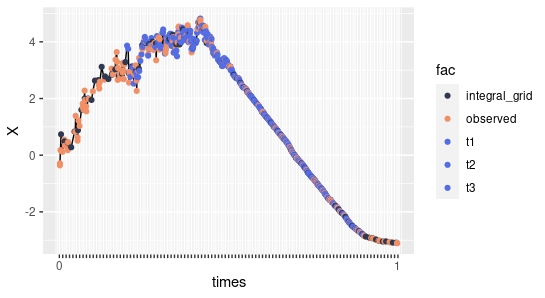
\includegraphics[width=0.48\textwidth]{Images/simul/all.jpeg}
	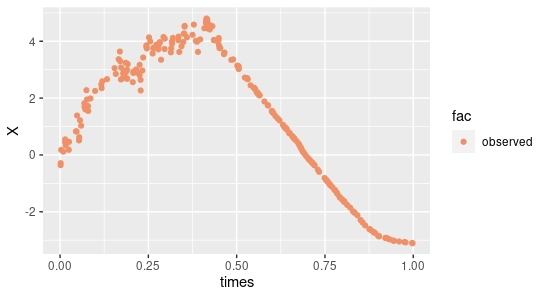
\includegraphics[width=0.48\textwidth]{Images/simul/observed.jpeg}

	\textbf{Lissage des données}

	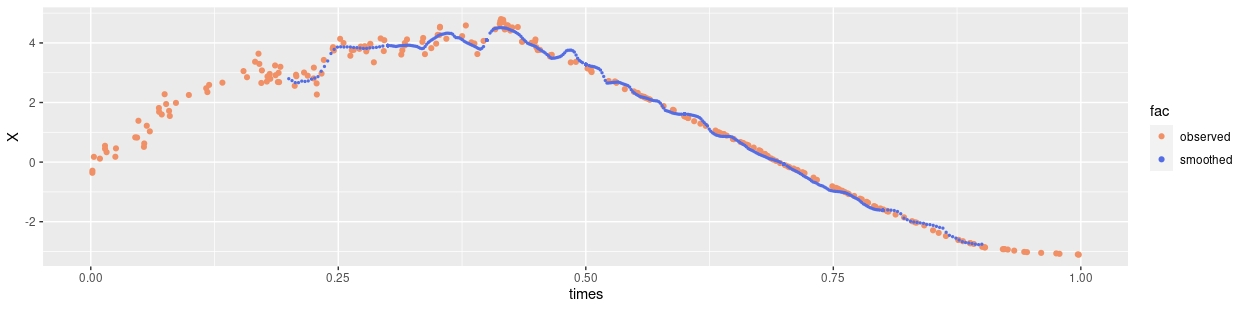
\includegraphics[width=0.96\textwidth]{Images/simul/smoothed.jpeg}
	\caption{Visualisation des données générées : $\lambda = 255, N = 200,$ 30 valeurs de $\Delta$}
\end{figure}


\subsection{Pré-Lissage}

Le pré-lissage des courbes a été fait en utilisant un lissge non paramétrique à noyaux\footnote{ainsi qu'un lissage utilisant des splines pénalisées, et des ondelettes mais on ne se concentrera sur les autres lissages qu'en Annexe \ref{annexe:prelissage_impact}}. Comme mentionné dans la section \ref{eq:h_cross_noyau_pre}, chaque courbe est lissée en utilisant une fenêtre par validation croisée avec la grille $\mathcal H= \{ 0.01 \dots 0.2 \}_{50}$ avec pour métrique une estimation du risque quadratique $\esperance{|\widehat Y_{(-i)} - Y|^2}$. On ne regarde pas de fenêtre au delà de $\Delta = 0.2$ car il serait difficile de justifier pour l'estimation de la régularité que l'on lisse en regardant plus de $20$\% du support alors que la régularité évolue sur l'ensemble de l'intervalle.

L'obtention de la fenêtre de lissage a été réalisée en réalisant une validation croisée sur une grille de fenêtre étalées sur une échelle de puissance entre $h_{min} = 2 / \widehat \lambda$ et $h_{max} = 1 / \widehat \lambda^{1/3}$.

\begin{align*}
	                                                 & \mathcal H = \bigl\{ h_k, \, k \in \llbracket 1, K \rrbracket \bigr\}
	\\
	\forall k \in \llbracket 1, K \rrbracket, \qquad & h_k = h_{min} e^{ - a \cdot k }
	\\
	\text{avec } \qquad                              & a = \frac{\log \left( h_{max} \right) - \log(h_{min})}{K}
	\\
	\textsf{de valeur max} \qquad                    & h_K = h_{max} = h_{min} e^{ - a \cdot K }
	\\
	\text{et } \qquad                                & K = 30
\end{align*}

Cela est dû au fait que $h^*_{\mathcal R_{\textsf{quadr}}} = \grandop{ \lambda^{- \frac 1 {1 + 2H_t}} }$ avec $0<H_t<1$, comme vu dans la section \ref{sec:regloc-prelissage}. De plus, on souhaite que dans notre fenêtre de lissage, en moyenne, se trouvent 2 points au minimum. 




% \section{Qualité de l'estimation des incréments quadratiques moyens}
% 
\newcommand{\thetaA}{\Theta_{1 \rightarrow \overset{3}{\underset {2}{}}}}
\newcommand{\cindexA}{_{1 \rightarrow \overset{3}{\underset {2}{}}}}
\newcommand{\thetaB}{\Theta_{\overset 1{\underset{2}{ }} \rightarrow3}}
\newcommand{\cindexB}{_{\overset 1{\underset{2}{ }} \rightarrow3}}
\newcommand{\thetaC}{\Theta_{1 \rightarrow 2 \rightarrow 3}}
\newcommand{\cindexC}{_{1 \rightarrow 2 \rightarrow 3}}
\newcommand{\notequiv}{\overset {\textsf{\faTimes}} \iff}
\newcommand{\yesequiv}{\overset {\textsf{\faCheck}} \iff}

Il y a différentes manières de définir les paramètres de régularité $\hat H_t$ et $\hat L_t$. En effet il est possible de définir $\hat H_t$ en utilisant $\hat \theta (t_1, t_2)$ mais aussi en utilisant $\hat \theta (t_2, t_3)$ ($\theta(t_1, t_3)$ est forcément utilisé\footnote{$\hat H_t$ ne serait même pas bien défini pour le couple $\theta(t_1, t_2)$, $\theta(t_2, t_3)$}). De même pour $\hat L_t$. On peut donc se demander quels sont les meilleurs $\theta(u,v)$ avec $u,v \in \{t_1, t_2, t_3\}$ à utiliser pour obtenir la meilleure estimation de $H_t$ et $L_t$ ainsi que leur $\Delta$ optimal associé pour l'estimation de ces paramètres.

\bigskip

Le problème est que le proxy $\theta$ est défini comme une espérance, et donc n'est pas observable. On ne peut donc pas directement comparer $\hat \theta(u,v) = \sum_i|\widehat X_i(u) - \widehat X_i(v)|^2$ et $\theta(u,v) = \esperanceloi X { |X(u) - X(v)|^2 }$, à moins d'avoir fait le calcul de l'expression explicite en connaissant la loi du processus initial.

\bigskip

On peut cependant comparer $\hat \theta(u,v)$ et $\widetilde \theta(u,v) = \frac 1 N \sum_i |X_i(u) - X_i(v)|^2$ qui est un estimateur de $\theta(u,v)$, et que l'on obtient aisément avec la simulation. On peut ainsi déterminer pour quelle valeur de $\Delta$ et quel couple $(u,v)$ on dispose de la meilleur estimation du $\tilde \theta$, qui est entre-autre le meilleur estimateur que l'on pourrait espérer de $\theta$. Le meilleur couple (au sens donné dans cette section) est pris comme étant les deux $\hat \theta(u,v)$ réalisant les risques minimaux par rapport au $\tilde \theta$ sur les 3 couples $(u,v)$ possibles.

\begin{table}[H]
	\centering
	\begin{tabular}{l|ll|}
		\cline{2-3}
		                                     & $\lambda < 120$                                                                                            & $\lambda \geq 120$                                                                 \\ \hline
		\multicolumn{1}{|l|}{$H_t < 0.6$}    & \multicolumn{1}{l|}{\begin{tabular}[c]{@{}l@{}}$\thetaC$\\ \\ \\ $\Delta^- \rightarrow 0.01$\end{tabular}} & \begin{tabular}[c]{@{}l@{}}$\thetaA$\\ \\ $\Delta^+ \rightarrow 0.2$\end{tabular}  \\ \cline{2-3}
		\multicolumn{1}{|l|}{$H_t \geq 0.6$} & \multicolumn{1}{l|}{\begin{tabular}[c]{@{}l@{}}$\thetaA$\\ \\ $\Delta^- \rightarrow 0.2$\end{tabular}}     & \begin{tabular}[c]{@{}l@{}}$\thetaC$\\ \\ $\Delta^+ \rightarrow 0.01$\end{tabular} \\ \hline
	\end{tabular}
	\caption{Tableau récapitulatif des $\Theta$ optimaux : Risque individuel sur $\tilde \theta(u,v)$}
	\label{tab:recap_theta_single}
\end{table}

% 
% \section{Qualité de l'estimation de la régularité locale}
% 
Les simulations de Monte Carlo permettent d'avoir accès directement à la véritable régularité de la courbe en chaque point. Nous allons dans l'étude du comportement du $\Delta$ essayer de tirer profit de cet avantage que ne possède pas le praticien qui utilise des données réelles.


\begin{table}[H]
    \centering
    \begin{tabular}{l|ll|}
        \cline{2-3}
                                              & $\lambda < 120$                                                                                                                                                                                                    & $\lambda \geq 120$                                                                                                                                        \\ \hline
        \multicolumn{1}{|l|}{$H_t \leq 0.65$} & \multicolumn{1}{l|}{\begin{tabular}[c]{@{}l@{}}$\yesequiv \mathcal R$\\ $\yesequiv \Delta^*$\\ $\Delta^- \downarrow 0.01$\end{tabular}}                                                                            & \begin{tabular}[c]{@{}l@{}}$\simeq \yesequiv \mathcal R$\\ $\notequiv \Delta^*$\\ $\Delta^+ \rightarrow [\leq 0.6] 0.1/0.2 [\geq 0.6]$\end{tabular}        \\ \cline{2-3}
        \multicolumn{1}{|l|}{$H_t > 0.65$}    & \multicolumn{1}{l|}{\begin{tabular}[c]{@{}l@{}}$\yesequiv \mathcal R$\\ $\notequiv \Delta^*$\\ \faExclamationTriangle $H=0.7 : \Delta^- = 0.02$\\ \faExclamationTriangle $H = 0.73 : \Delta^- = 0.2$\end{tabular}} & \begin{tabular}[c]{@{}l@{}}$\thetaA$\\ \faExclamationTriangle $H=0.7 : \Delta^+ = 0.02$\\ \faExclamationTriangle $H = 0.73 : \Delta^+ = 0.2$\end{tabular} \\ \hline
    \end{tabular}
    \caption{Tableau récapitulatif des $\Delta$ optimaux : Risque sur $H_t$}
    \label{tab:recap_delta_H}
\end{table}



\section{Qualité de l'estimation des couples d'incréments utilisés dans l'estimation de la régularité}
\label{sec:choix_risque_couple}

\info{
	on rappelle les notations suivantes :

	\begin{itemize}
		\item vrai : $\theta = \mathds E \bigl[ \, f(X) \, \bigr]$
		\item intangible/inobservable : $\widetilde \theta = \frac 1 N \sum_i f(X_i)$
		\item observable : $\widehat \theta = \frac 1 N \sum_i f(\widehat X_i)$
	\end{itemize}
}

L'estimation des paramètres de régularité locale en $t_2$, $H_{t_2}$ et $L_{t_2}$, utilise les incréments quadratiques $\theta$ entre les différents points $t_1, t_2, t_3$ dans un voisinage de diamètre $\Delta$ autour de $t_2$. 

\question{
	Quelle quantité est-il judicieux d'évaluer pour estimer au mieux la régularité locale en $t_2$ ? Doit-t-on regarder la qualité de l'approximation de $\theta$ (qui est une espérance) car il est utilisé pour tous les estimateurs ? Ou doit-on regarder la qualité de l'approximation de $H_{t_2}$ et $L_{t_2}$ car ce sont les quantités qui nous intéressent ? Ou bien les deux ? 
}

Le choix du bon critère d'évaluation est d'une grande importance. Il faut se rappeler l'objectif que l'on cherche à atteindre : déterminer une procédure (simple si possible) de détermination de l'hyper-paramètre $\Delta$ utilisé pour l'estimation de la régularité locale en fonction de quantités facilement estimables, ou directement observables par le praticien. En observant que $L$ est estimée par une expression impliquant $\theta$ et $\Delta^{2 H}$, une estimation précise de $H$ paraît plus cruciale pour la bonne estimation des deux quantités. Bien qu'il existe certainement un compromis entre la bonne estimation de $H$ et de $L$ qui fournit une meilleure estimation adaptative des quantités qui nous intéressent, il est certainement plus probable de dériver une procédure de sélection de $\Delta$ simple à implémenter pour le praticien en se basant sur la qualité de l'estimation d'une unique quantité.

\question{
	Doit-t-on se concentrer sur l'estimation de $H$ ou de $\theta$ ?
}

Les incréments sont des quantités importantes dans l'estimation de la régularité, utilisées à la fois pour l'estimation de $H$ et de $L$, l'approche que l'on considère se base sur cette remarque. Nous allons donc chercher à déterminer un $\Delta$ adapté à l'estimation des incréments quadratiques. Toutefois, il y a plusieurs possibilités de $u,v \in J_\Delta(t_2)$ que l'on peut considérer pour l'estimation de $H$ et $L$. C'est pourquoi nous décidons de considérer les \emph{couples} d'incréments utilisés pour l'estimation de $H$. Ainsi en posant :

\begin{minipage}{0.5\textwidth}
	\begin{equation*}
		\thetaA = \begin{bmatrix} \theta(t_1, t_3) \\ \theta(t_1, t_2) \end{bmatrix}
	\end{equation*}
\end{minipage}
\hfill
\begin{minipage}{0.5\textwidth}
	\begin{equation*}
		\thetaB = \begin{bmatrix} \theta(t_1, t_3) \\ \theta(t_2, t_3) \end{bmatrix}
	\end{equation*}
\end{minipage}

\smallskip

L'estimateur du paramètre de régularité $H_t$ peut se ré-écrire comme :

\smallskip


\begin{equation*}
	\widehat H_t : \Theta = \begin{bmatrix} \Theta_1 \\ \Theta_2 \end{bmatrix} \longmapsto \frac{ \log \widehat \Theta_1 - \log \widehat \Theta_2 }{2 \log 2}
\end{equation*}

\smallskip

Le problème c'est qu'on ne dispose pas de la véritable valeur de $\theta(u,v)$, on pourrait exploiter le fait que l'on dipose d'un mouvement brownien multi-fractionnaire qui a été étudié de façon extensive dans la littérature, mais on décide de ne pas l'utiliser pour adopter une approche plus proche d'un cadre général. 
Le meilleur estimateur que l'on puisse espérer atteindre est $\bigl(\hat H_t( \widetilde \thetaA)$ ou $\hat H_t( \widetilde \thetaB)\bigr)$, estimateur utilisant les courbes pleinement observées et non bruitées. On va donc s'intéresser désormais à l'erreur d'estimation conjointe des deux $\theta(u,v)$ utilisés dans l'estimation de $H_t$ par rapport à cet estimateur en quelque sorte \og idéal \fg de $\theta$ comme critère de sélection du diamètre $\Delta$.

\begin{figure}[H]
	\centering
	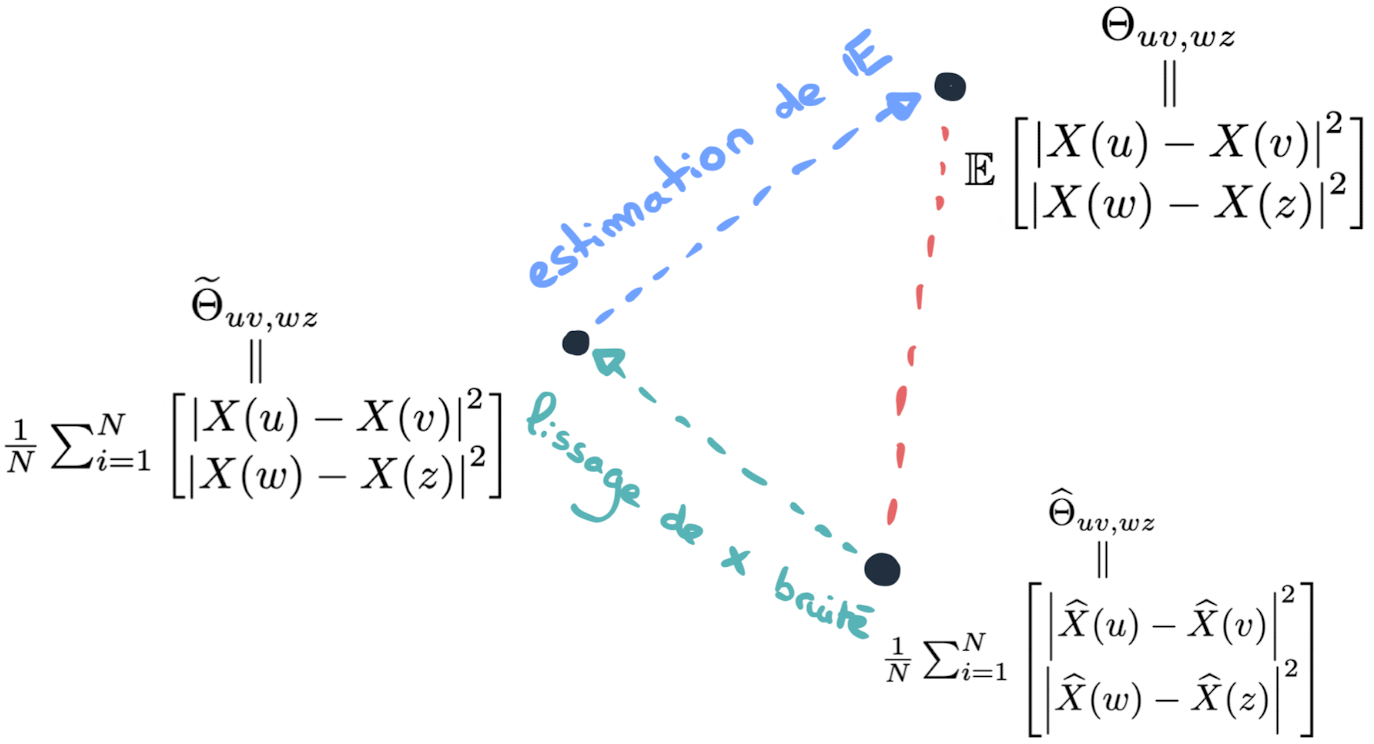
\includegraphics[width=0.7\textwidth]{Images/sketches/theta_biais.png}
	\caption{Schéma représentant les différents biais et approximations du couple d'incréments}
	\label{fig:sketch_theta_biais}
\end{figure}


Pour cela on considère la distance euclidienne usuelle pour des vecteurs de $\R 2$

$$R(\Theta, \Delta) = \distnorme 2 {\widehat \Theta(\Delta)} {\widetilde \Theta(\Delta)}$$

et on nomme $R\cindexA(\Delta) = R( \thetaA , \, \Delta \, )$ et $R\cindexB(\Delta) = R( \thetaB, \, \Delta \, )$

\begin{table}[H]
	\centering
	\begin{tabular}{l|ll|}
		\cline{2-3}
		                                     & $\lambda < 120$                                                                                                                                                                                                           & $\lambda \geq 120$                                                                             \\ \hline
		\multicolumn{1}{|l|}{$H_t < 0.6$}    & \multicolumn{1}{l|}{\begin{tabular}[c]{@{}l@{}}$\yesequiv \mathcal R, \Delta^*$\\ $\Delta^*_- = 0.01$\end{tabular}}                                                                                                       & \begin{tabular}[c]{@{}l@{}}$\thetaB$\\ $\Delta^*_+ = 0.2$\end{tabular}                         \\ \cline{2-3}
		\multicolumn{1}{|l|}{$H_t \geq 0.6$} & \multicolumn{1}{l|}{\begin{tabular}[c]{@{}l@{}}$\thetaB$\\ $\Delta^*_- = 0.2$\\ \\\faExclamationTriangle $H=0.7 : \Delta^- = 0.01 \oplus \yesequiv \mathcal R$\\ \\\faExclamationTriangle $H=0.8 : \thetaA$\end{tabular}} & \begin{tabular}[c]{@{}l@{}}$\yesequiv \mathcal R, \Delta^*$\\ $\Delta^*_+ = 0.01$\end{tabular} \\ \hline
	\end{tabular}
	\label{tab:recap_delta_eucl_h_global_pour_lambda_sup}
	\caption{Tableau récapitulatif des $\Delta$ optimaux : Risque euclidien sur $\tilde \Theta$ | fenêtre de prélissage globale pour $\lambda \geq 120$}
\end{table}


\subsubsection{Comparaison entre les 3 différentes méthodes de lissage sur l'estimation des couples $\Theta$}

\question{Peut on quantifier le biais introduit par le lissage en utilisant les ondelettes sur l'estimation de la régularité locale ?}

\editlater{regarder ce que ça donne, en utilisant les différents théorèmes et bornes disponibles sur les ondelettes pour un processus Holder LORSQUE J AI LE TEMPS - certainement en Septembre}

\section{Détermination d'un critère de choix du diamètre $\Delta$ des intervalles à considérer pour l'estimation de la régularité locale}


Maintenant que l'on a déterminé que l'on souhaite travailler sur un les couples $\thetaB = \begin{bmatrix} \theta(t_1, t_3) \\ \theta(t_2, t_3) \end{bmatrix}$ et $\thetaA = \begin{bmatrix} \theta(t_1, t_3) \\ \theta(t_1, t_2) \end{bmatrix}$, il nous faut déterminer un critère pour déterminer quel couple est plus judicieux pour la méilleure estimation en pratique des paramètres de régularité locale.

L'heuristique est la suivante : dans nos simulations, on a le luxe de pouvoir faire 200 simulations de monte carlo et obtenir le $\Delta^*$ le plus proche du $\Delta$ optimal pour estimer la régularité. Dans la pratique, obtenir un tel $\Delta$ optimal n'est pas réaliste, on se trouvera soit un peu en dessous, soit un peu au dessus. L'idée est donc de favoriser le couple de $\theta(u,v)$ qui possède le plus grand plateau autour du $\Delta^*$ pour le risque quadratique \emph{si l'écart de risque quadratique entre les deux couples n'est pas trop important}. Si l'un est beaucoup plus performant que l'autre, on choisira le plus performant. Mais si la performance des deux est à peu près équivalente, autant sélectionner celui qui dans la pratique (sans avoir 200 réplications indépendantes) nous donnera le plus de flexibilité sur l'erreur commise en sélectionnant un $\Delta$ autour du $\Delta^*$ dû à la fluctuation statistique.

\subsection{Détermination d'un seuil pour l'équivalence de risque quadratique}

Il nous faut maintenant déterminer ce que l'on considère comme étant deux risques "équivalents". Pour cela on va déterminer pour différentes valeurs du véritable $H$ le seuil $\varepsilon$ sur le risque tel que $R\cindexA(\Delta + \delta) + \varepsilon$ induit une erreur d'au maximum $10$\% sur le H estimé. On viendra ensuite déterminer les $\delta$ qui en moyenne correspondent à ce seuil $\varepsilon$ pour les différentes valeurs de $H$.

\subsection{Détermination du meilleur couple à risque \og équivalent \fg}

\subsubsection{en utilisant les pentes}


Une méthode possible serait de définir la pente à gauche et la pente à droite de la façon suivante :

\begin{align*}
	a_g : \Delta, \delta & \mapsto \frac{R(\Delta) - R(\Delta - \delta)}{\delta} \\
	a_d : \Delta, \delta & \mapsto \frac{R(\Delta + \delta) - R(\Delta)}{\delta}
\end{align*}
On peut définir les pénalisations suivantes pour déterminer le meilleur couple à risque équivalent en terme de plateau, en pénalisant les larges différence entre la pente à gauche et à droite :

\begin{equation*}
	m_q(\Delta, \delta) = \frac{a_g^2(\Delta, \delta) + a_d^2(\Delta, \delta)}{2}
\end{equation*}

\subsubsection{en utilisant les valeurs de risque}
une autre méthode est de regarder :

\begin{align*}
	R_2(\Delta^*_2) & \geq R_1(\Delta^*_1)                                      \\
	dR              & = \bigl\vert R_1(\Delta^*_1) - R_2(\Delta^*_2) \bigr\vert
\end{align*}
on compare désormais les valeurs de :

\begin{align*}
	r_g^{[2]} & = R_2(\Delta^*_2 - \delta) - dR \\
	r_d^{[2]} & = R_2(\Delta^*_2 + \delta) - dR
\end{align*}
aux valeurs

\begin{align*}
	r_g^{[1]} & = R_1(\Delta^*_1 - \delta) \\
	r_d^{[1]} & = R_1(\Delta^*_1 + \delta)
\end{align*}
avec le critère de sélection suivant :

\begin{equation*}
	\argmin \bigl( \frac{r_g^{[1]} + r_d^{[1]}}{2}, \frac{r_g^{[2]} + r_d^{[2]}}{2}  \bigr)
\end{equation*}
Pour pénaliser les solutions où la pente à gauche est très différente de la pente à droite en magnitude, on peut considérer d'élever $r_g$ et $r_d$ au carré.

\begin{equation*}
	\argmin \bigl( \frac{(r_g^{[1]})^2 + (r_d^{[1]})^2}{2}, \frac{(r_g^{[2]})^2 + (r_d^{[2]})^2}{2}  \bigr)
\end{equation*}
\subsubsection{résultat}

\warn{
	Il est important de garder en tête le modèle dans lequel on s'est placé pour étudier le comportement du $\Delta$. La recommendation qui est faite pour la sélection du $\Delta$ est valable pour :

	\begin{itemize}
		\item $\operatorname{FAR}(1)$ construit à partir d'un $\operatorname{mfBm}(H, L)$
		\item la régularité donnée par $H(t)$, qui dans notre cas est $\mathcal C^\infty$ sur $[0,1]$
		\item le noyau de la relation auto-régressive $\beta$ est une fonction de classe $\mathcal C^{\infty}$ sur $]0, 1]$ et continue en $0$
		\item La dérivée de $H$ est $H' :t \mapsto \frac{2 e ^{-5(t-0.5)}}{\left(1 + e ^{-5(t-0.5)}\right)^2}$, la variation maximale de la régularité est atteinte en $\argmax\limits_{t \in [0,1]} H'(t) = \frac 1 2$ avec $H'(\frac 1 2)=\frac 1 2$
		\item La régularité est monotone et strictement croissante sur $[0,1]$
	\end{itemize}

	Trop s'éloigner de ces hypothèses pourrait demander d'analyser de nouveau le comportement du $\Delta$ dû aux propriétés de certaines de ces quantités qui aurrait pu influencer le résultat.
}


